Previamente, no nível base (Seção \ref{expbase}), a efetividade prática das estratégias propostas foi experimentalmente verificada pela avaliação direta de suas curvas de aprendizado, incluindo a adoção do meta-aprendiz como alternativa ao uso de um algoritmo de aprendizado específico.
No nível meta, entretanto, a avaliação se concentra na verificação da ocorrência de aprendizado, isto é, se a capacidade preditiva do meta-aprendiz supera os métodos de referência: Def (ranqueamento médio), Maj (predição da classe majoritária) e Alea (predição aleatória).
O algoritmo de recomendação foi avaliado com foco nas PCT, pelo fato de sua implementação disponível viabilizar a predição de ranqueamento (Seção \ref{rankalg}).
No entanto, outros algoritmos também foram adotados como meta-aprendizes na tarefa de predição do melhor algoritmo de aprendizado para uma dada estratégia de amostragem ativa, na Seção \ref{recalg}.
Adicionalmente, na Seção \ref{metaatts}, a relevância dos meta-atributos é investigada.

O mesmo esquema de reconsideração de escolhas do sistema de recomendação da Seção anterior foi adotado:
o processo de rotulação foi considerado como dois períodos de consultas que correspondem às suas metades do processo de rotulação.
Logo, para cada estratégia, duas metapredições foram feitas.

\subsection{Ranqueamento de algoritmos de aprendizado}\label{rankalg}
As diferenças estatisticamente significativas entre PCT e Def foram reveladas pelo teste de Wilcoxon aplicado a 90 valores de correlação entre ranqueamentos esperados e preditos.
Esses valores correspondem aos testes do procedimento LOO (\textit{Leave-One-Out} - Seção \ref{testestmeta}) aplicado a toda a coleção de conjuntos de dados.
O nível de significância estatística é dado na Figura \ref{corrmeta}, onde cada linha corresponde a um experimento completo, sendo que, em cada experimento, uma estratégia diferente foi adotada.
O número sobrescrito indica a faixa de orçamentos: ``HTUeuc\textsuperscript{1}'', por exemplo, indica que a predição do ranqueamento é referente às primeiras 50 consultas;
``HTUeuc\textsuperscript{2}'' remete às 50 últimas consultas da mesma estratégia.
\input images/metacorr

O meta-aprendiz PCT obteve valores superiores à referência Def com todas as 28 estratégias, a maioria com diferenças estatisticamente significativas, reforçando assim a constatação de superioridade do sistema de recomendação.

Na metade inferior da figura, os valores de correlação são sistematicamente mais baixos para ambos metaclassificadores e muito próximos de zero para Def.
Essa metade corresponde às últimas 50 consultas do período de aprendizado (sobrescrito 2).
Supõe-se que, à medida que o aprendizado avança, a colocação média de cada algoritmo de aprendizado (aprendiz ativo) se torna mais próxima das demais, levando a um ranqueamento médio pouco representativo - conforme previamente ilustrado pela crescente intersecção entre as faixas na Figura \ref{curvasrankbands}.
Apesar dessa crescente dificuldade, nota-se também que, na segunda metade, o meta-aprendiz proposto se distingue ainda mais de Def, pois os $p$-valores são mais baixos, ocasionando uma maior frequência de $\alpha=0,01$ (símbolo *) que na metade superior.
Sucintamente, no panorama geral, PCT superou Def.

Consequentemente, é possível afirmar que, considerando a medida de desempenho adotada no nível base ($\mu_{\kappa}$) e dada a coleção de conjuntos de dados e os algoritmos adotados, para a maioria das estratégias \destaque{o meta-aprendiz foi capaz de induzir modelos que efetivamente representam conhecimento presente na relação entre os meta-atributos propostos e as metaclasses}\footnote{Desde que a coleção contenha mais do que um conjunto de um mesmo domínio (conforme demonstrado posteriormente no Apêndice \ref{apflu})}; em oposição ao que seria esperado se os modelos houvessem sido gerados ao acaso.

A avaliação experimental prossegue, na Seção \ref{recalg}, com a inclusão dos algoritmos RoF (\textit{Rotation Forest}), RFw (\textit{Random Forest}) e ABoo (\textit{AdaBoost}) enquanto meta-aprendizes, visando a comparação de desempenho no nível meta na tarefa de predição de classes.

\subsection{Recomendação de algoritmos de aprendizado}\label{recalg}
A recomendação do melhor algoritmo dis\-tan\-cia-se da predição de ranqueamentos e a\-pro\-xi\-ma-se da tarefa de classificação.
Ela visa a recomendação do melhor algoritmo apenas, descartando informações sobre as demais colocações.
Diferentemente da abordagem metodológica da Seção \ref {rankalg}, o método de validação LOO, e o subsequente teste de significância estatística, não puderam ser utilizados na comparação entre os algoritmos PCT, RoF, RFw e ABoo e as referências Maj e Alea - dada a natureza do experimento. Mais detalhes foram expostos previamente na Seção \ref{testestmeta}.

A acurácia média e o desvio padrão de cada algoritmo utilizado como meta-aprendiz, resultantes de dez execuções de validação cruzada em dez partes, são apresentados na Figura \ref{accmeta}.
\begin{figure}
\centering
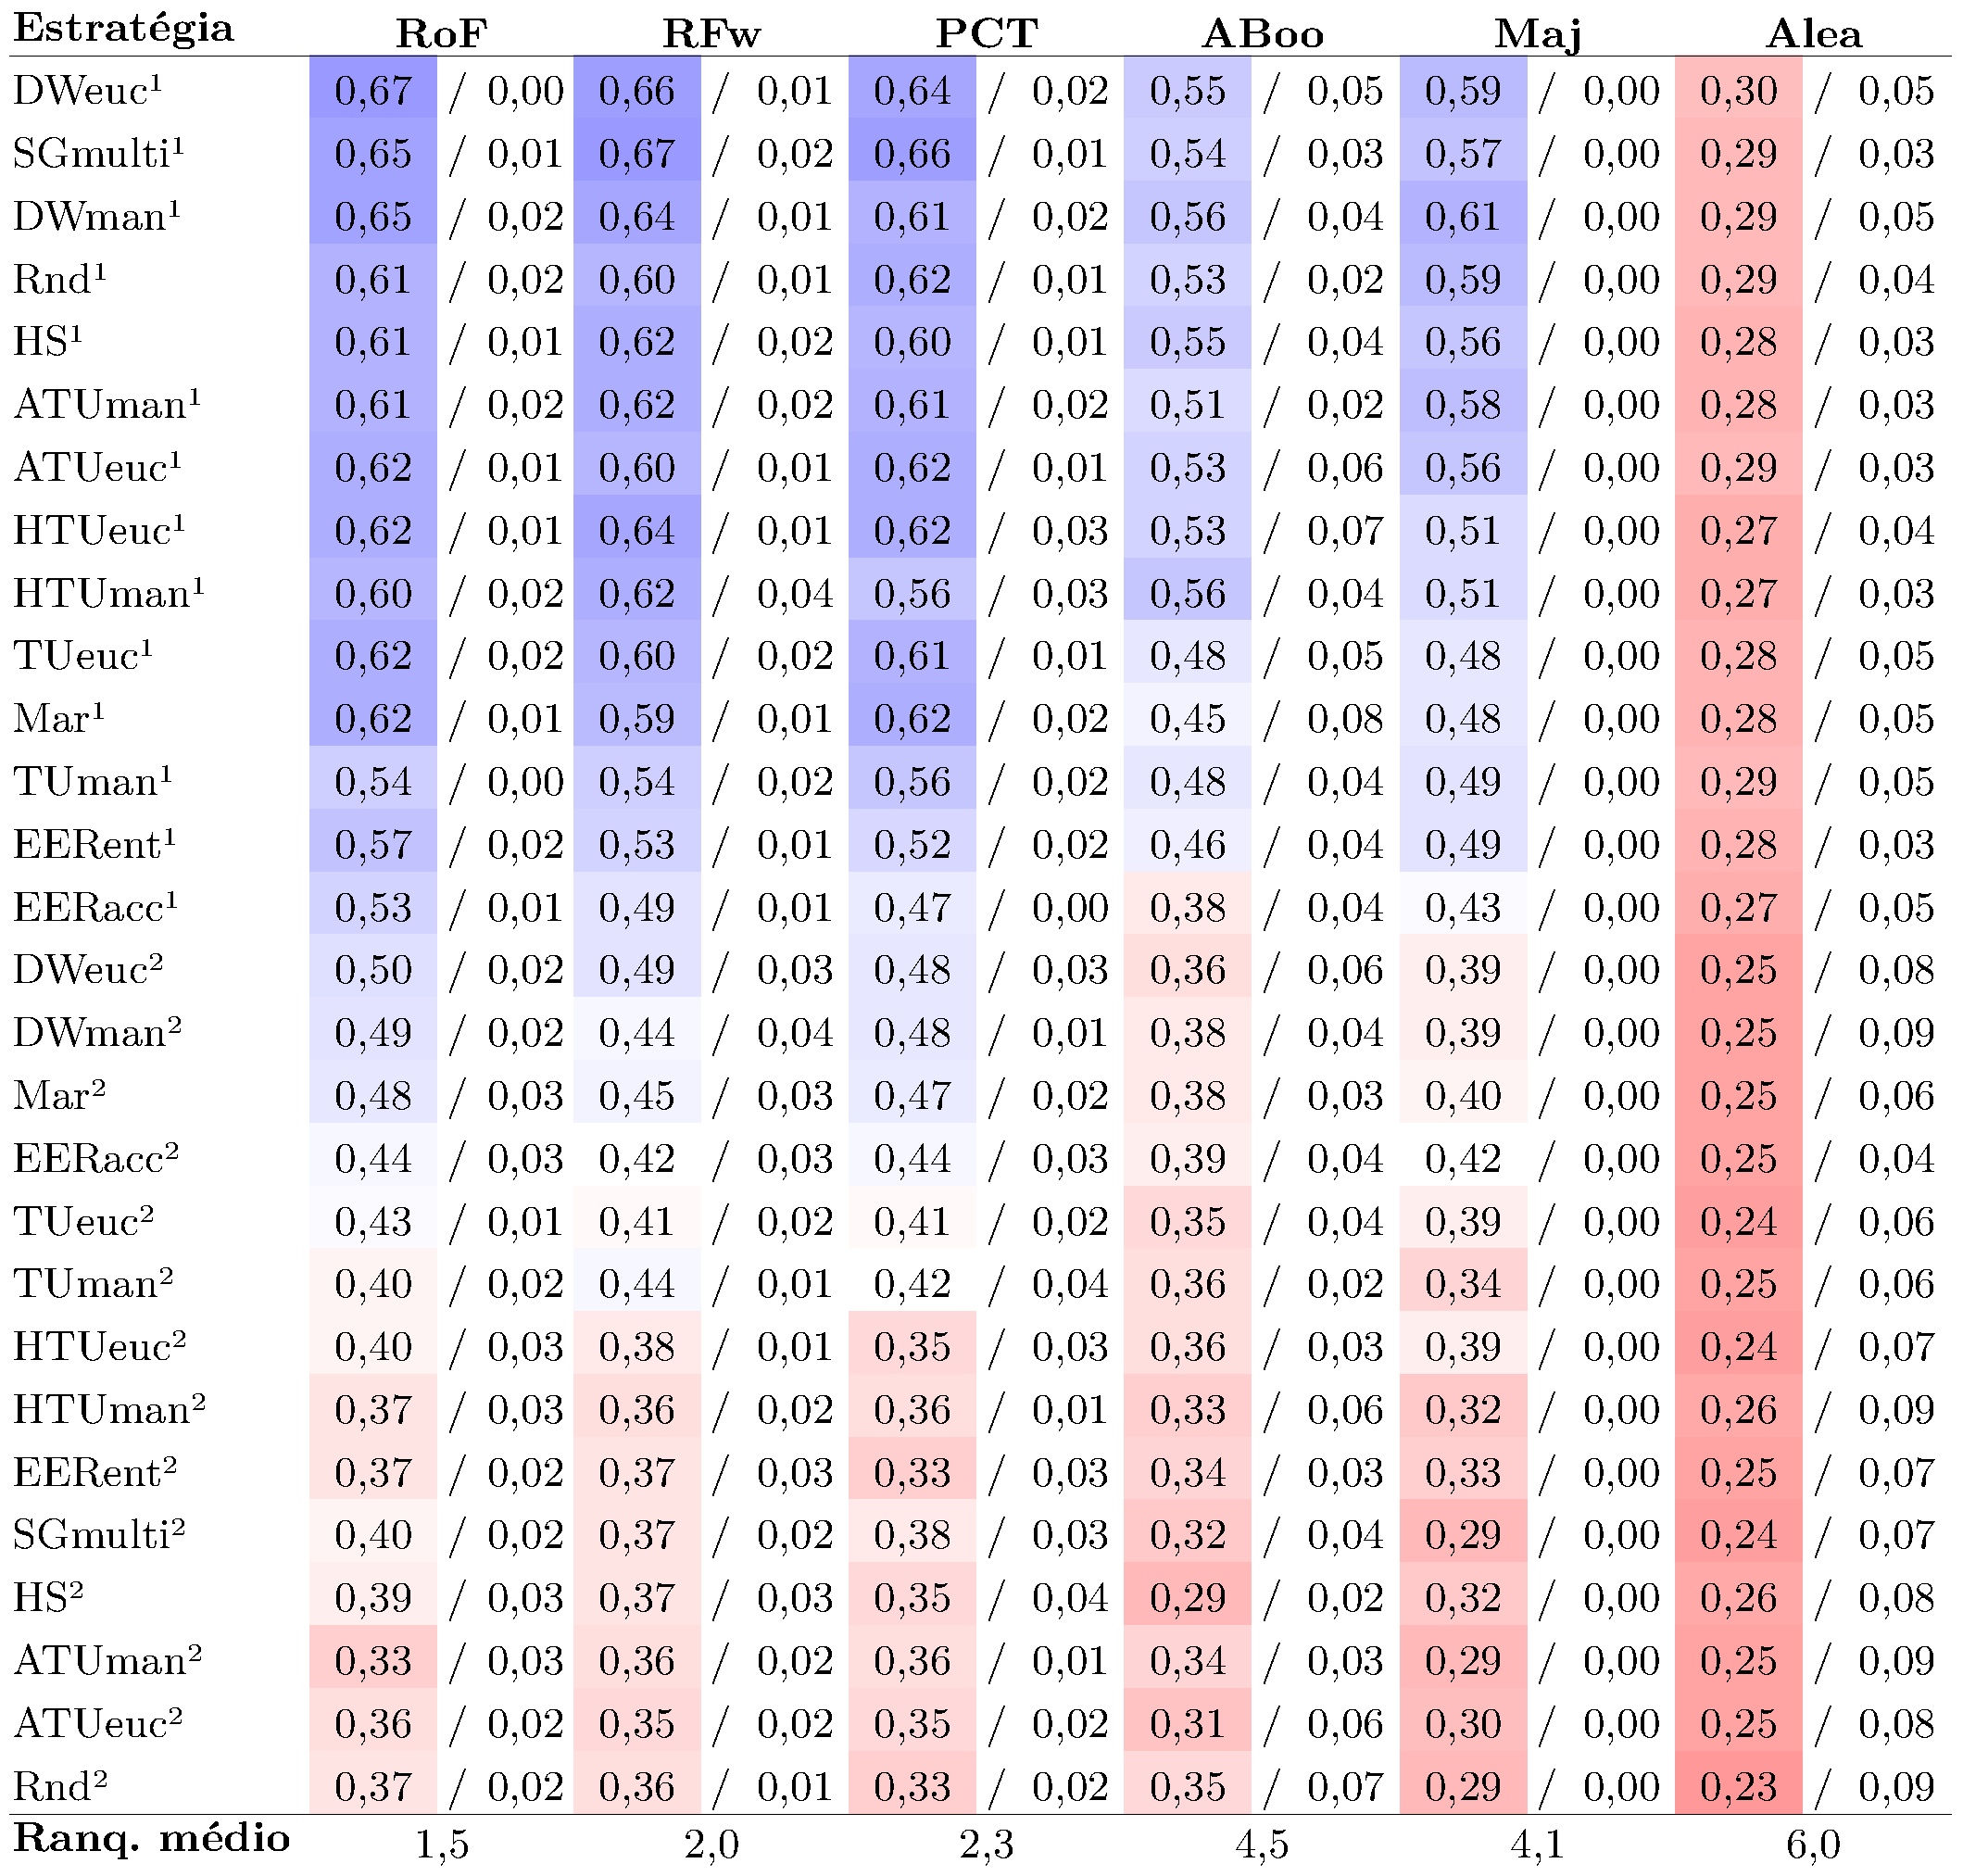
\includegraphics[scale=0.4]{images/metaacc.pdf}
% acc: 10x10-fold
% teste: sem teste
\caption[Comparação da acurácia na predição do melhor algoritmo de aprendizado.]{Comparação da acurácia (média/desvio padrão) na predição do melhor algoritmo de aprendizado.
\textit{Obs.: uma boa colocação no ranqueamento médio não implica em generalidade dos resultados, pois todas as linhas são altamente correlacionadas.}}
\label{accmeta}
\end{figure}
As linhas estão ordenadas a começar pelas acurácias mais altas.
Essa ordenação praticamente corresponde ao decrescimento dos valores para Maj, que representa a proporção de exemplos da metaclasse majoritária. Essa proporção influencia diretamente o patamar das demais acurácias.

% Uma peculiaridade dessa disposição é a concentração das cinco estratégias agnósticas no final da lista - situação similar à da ordenação por correlação, na Figura \ref{corrmeta}.
% Tais estratégias levaram a metaconjuntos mais balanceados no estágio mais avançado do período de consultas considerado (sobrescrito 2).
% Essa constatação sugere que alguns algoritmos de aprendizado são preferíveis a outros para uma dada estratégia não agnóstica.
% 
% No caso de exemplos consultados por estratégias sem aprendiz, ou, em menor grau, consultados da forma agnóstica de SGmulti, sempre a mesma sequência de exemplos é gerada, independentemente do algoritmo de aprendizado adotado.
% Dado que, nesse caso, o conjunto de treinamento é sempre o mesmo, essa tarefa é mais próxima da recomendação de algoritmos em aprendizado passivo do que em AA.
% Adicionalmente, por definição, estratégias sem aprendiz não requerem a adoção de um algoritmo de aprendizado.
% Consequentemente, elas poderiam prescindir do sistema de recomendação proposto caso a disponibilidade de um modelo preditivo durante o aprendizado não fosse imposto pelo cenário da aplicação.
% Logo, em certos cenários, os desempenhos do sistema de recomendação em estratégias sem aprendiz aqui reportados podem ser irrelevantes.

Tendo em vista os ranqueamentos médios, na última linha da figura, com exceção de ABoo, os meta-aprendizes alternativos obtiveram desempenho superior ao obtido pelo algoritmo PCT.
Isso favorece uma avaliação positiva do sistema de recomendação, pois o desempenho preditivo de PCT já havia sido reportado, na Seção \ref{rankalg}, com superioridade estatisticamente significativa com relação à referência Def.
Logo, é razoável estender essa constatação a RoF e RFw.
A validade dos valores de acurácia é reforçada pelos valores relativamente baixos de desvio padrão, quando consideradas as diferenças entre as médias atingidas pelos algoritmos alternativos e as médias atingidas pelos algoritmos de referência.
De fato, a superioridade dos meta-aprendizes é confirmada, de maneira mais clara, e incluindo ABoo, por meio de medidas que equilibrem o peso de todas as classes, como a acurácia balanceada e $\kappa$.

A relativa manutenção do comportamento dos valores de ranqueamento médio nas três figuras \ref{accmeta}, \ref{kappameta} e \ref{accbalmeta} aponta para a existência de redundância pelo menos parcial entre as suas respectivas medidas: acurácia, acurácia balanceada e $\kappa$.
Por simplicidade, apenas a medida $\kappa$ é reportada nas seções subsequentes, pois ela tem a vantagem de considerar a possibilidade do algoritmo acertar ao acaso, ou seja, ela já incorpora em seu valor a comparação com os métodos de referência.
Isso pode ser comprovado pelo desempenho praticamente nulo nas duas últimas colunas, referentes a esses métodos, na Figura \ref{kappameta}.
\begin{figure}
\centering
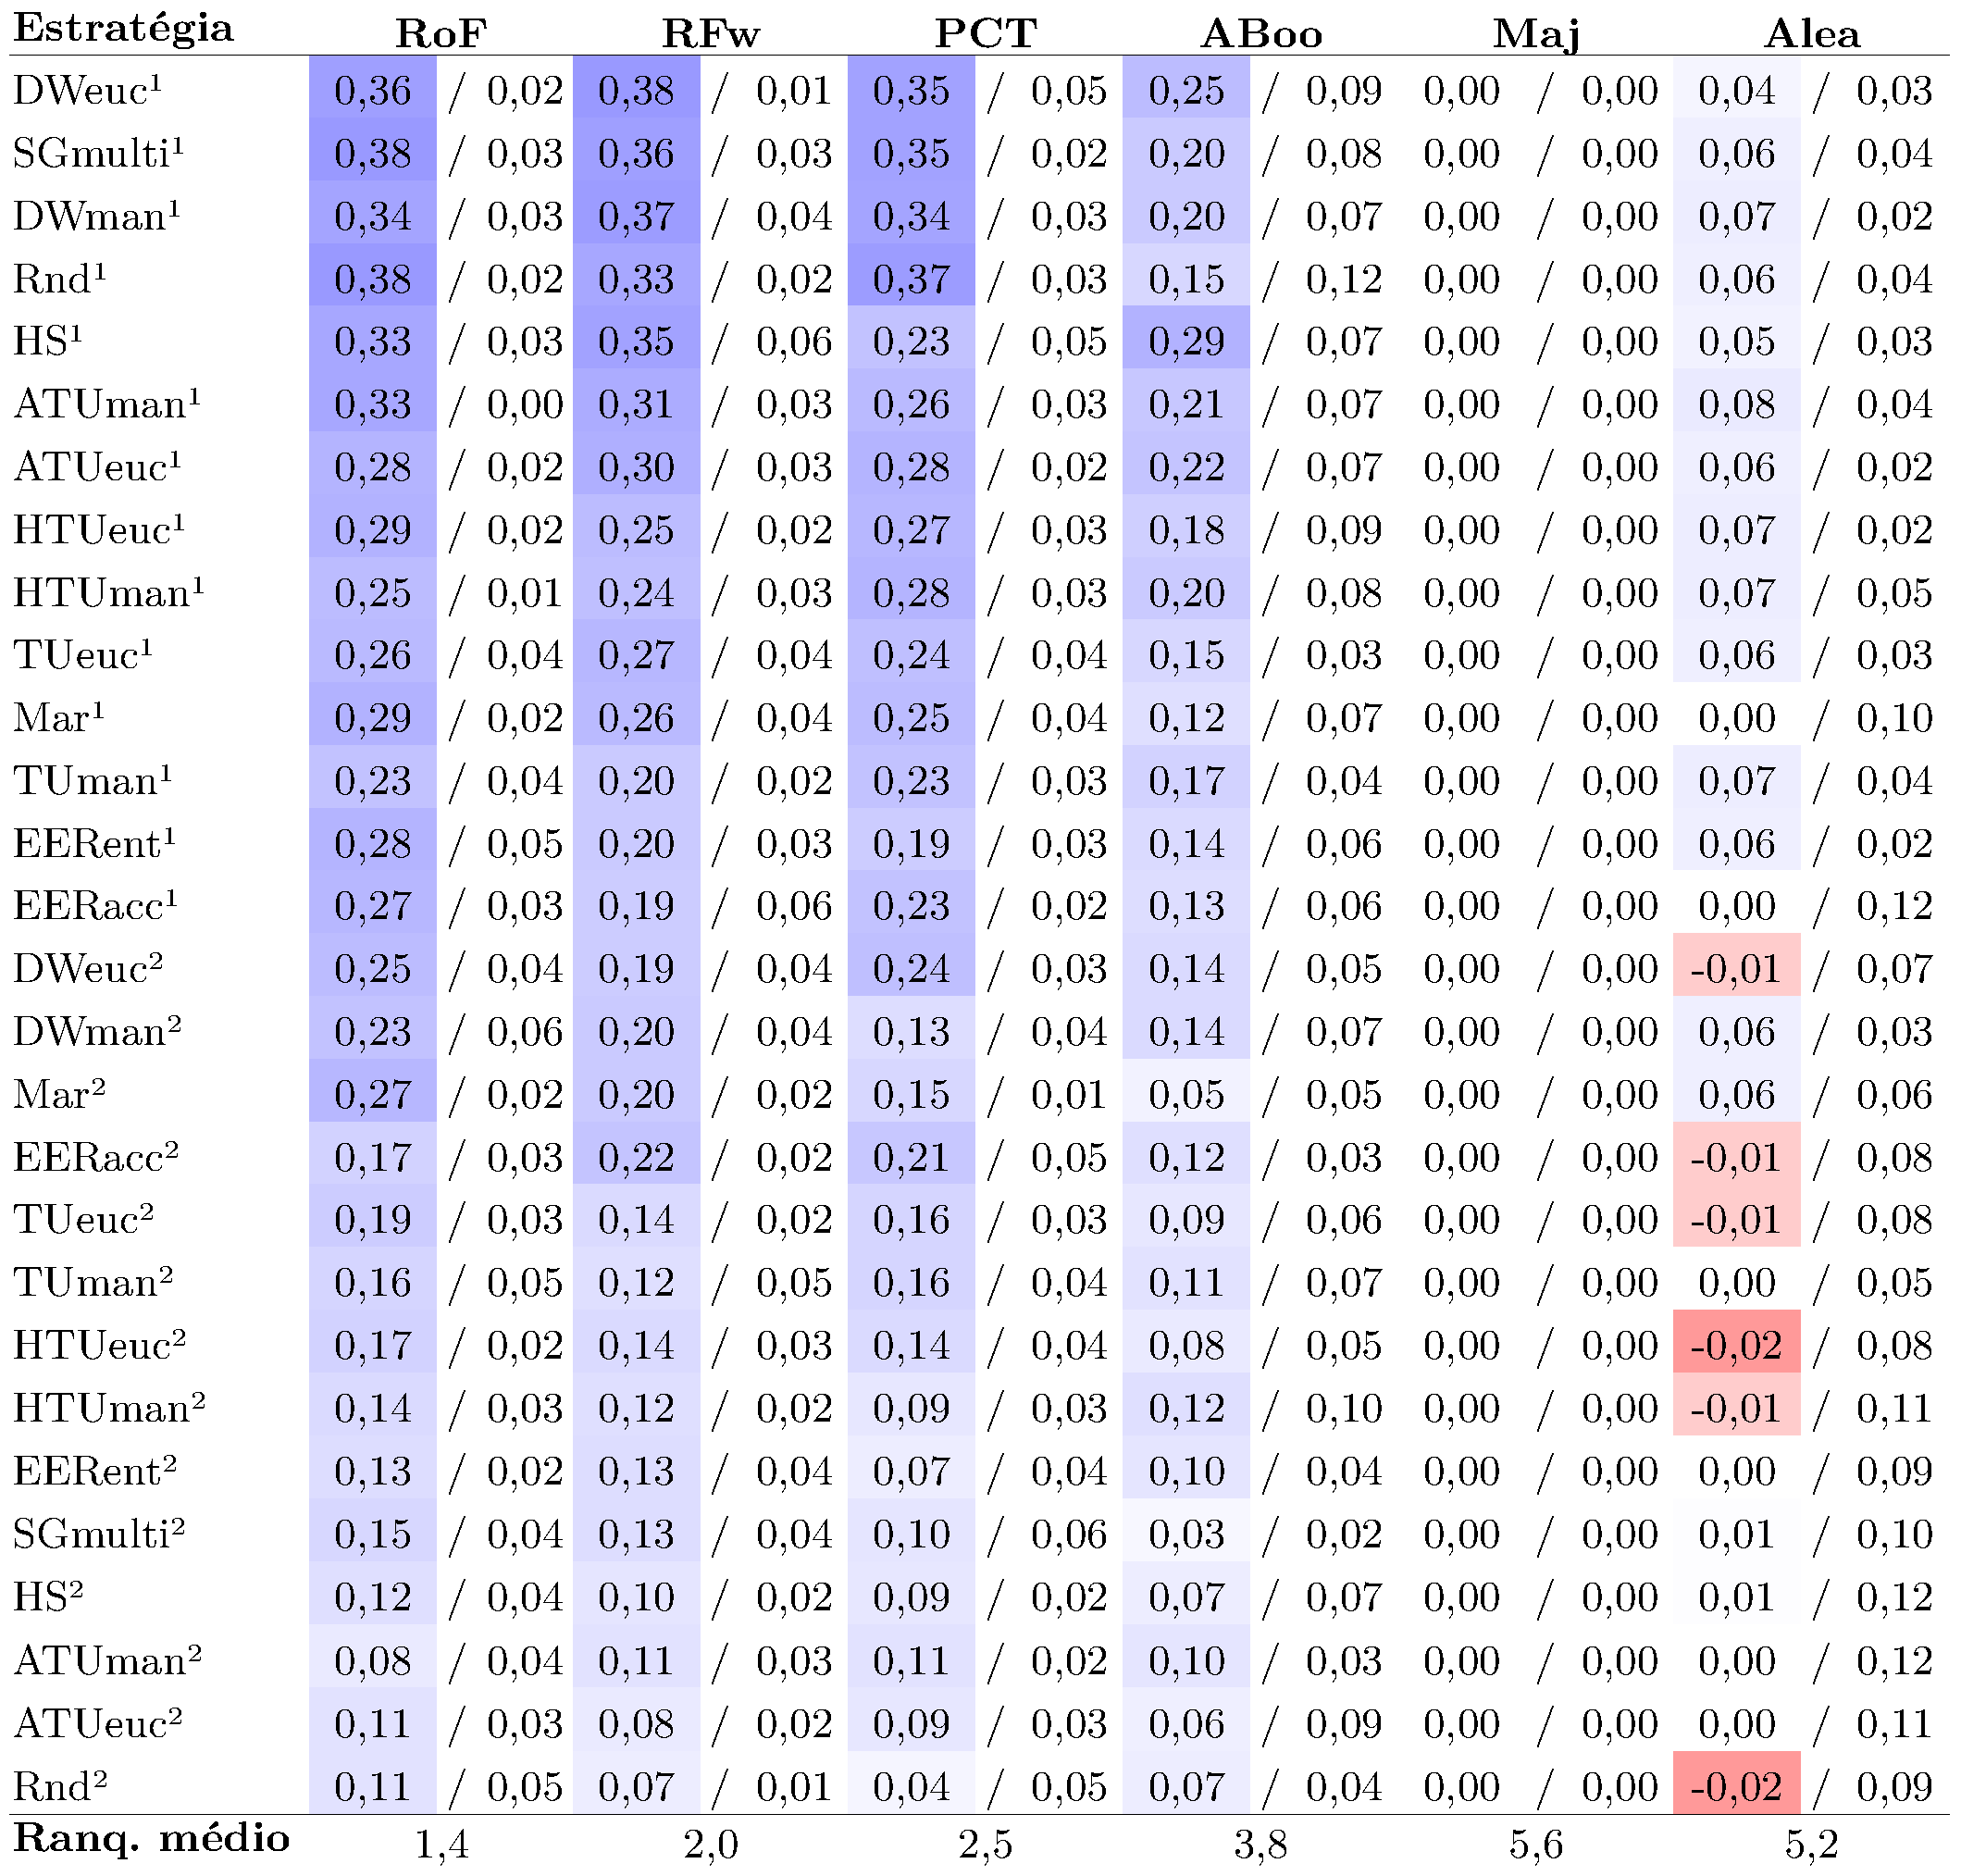
\includegraphics[scale=0.4]{images/metakap.pdf}
\caption[Comparação de $\kappa$ na recomendação do melhor algoritmo de aprendizado.]{Comparação de $\kappa$ (média/desvio padrão) na recomendação do melhor algoritmo de aprendizado.
\textit{Detalhes na Figura \ref{accmeta}.}}
\label{kappameta}
\end{figure}
Na mesma figura, é possível notar novamente a superioridade das colocações médias de RoF e RFw sobre PCT.

Com relação à acurácia balanceada, apenas dois dos meta-aprendizes foram superados em algum momento por uma das referências, conforme pode ser visto na Figura \ref{accbalmeta}:
PCT com a estratégia DWman obteve menor acurácia balanceada do que Alea; e, ABoo com as estratégias EERacc e DWman obteve menor acurácia balanceada do que Alea.
\begin{figure}
\centering
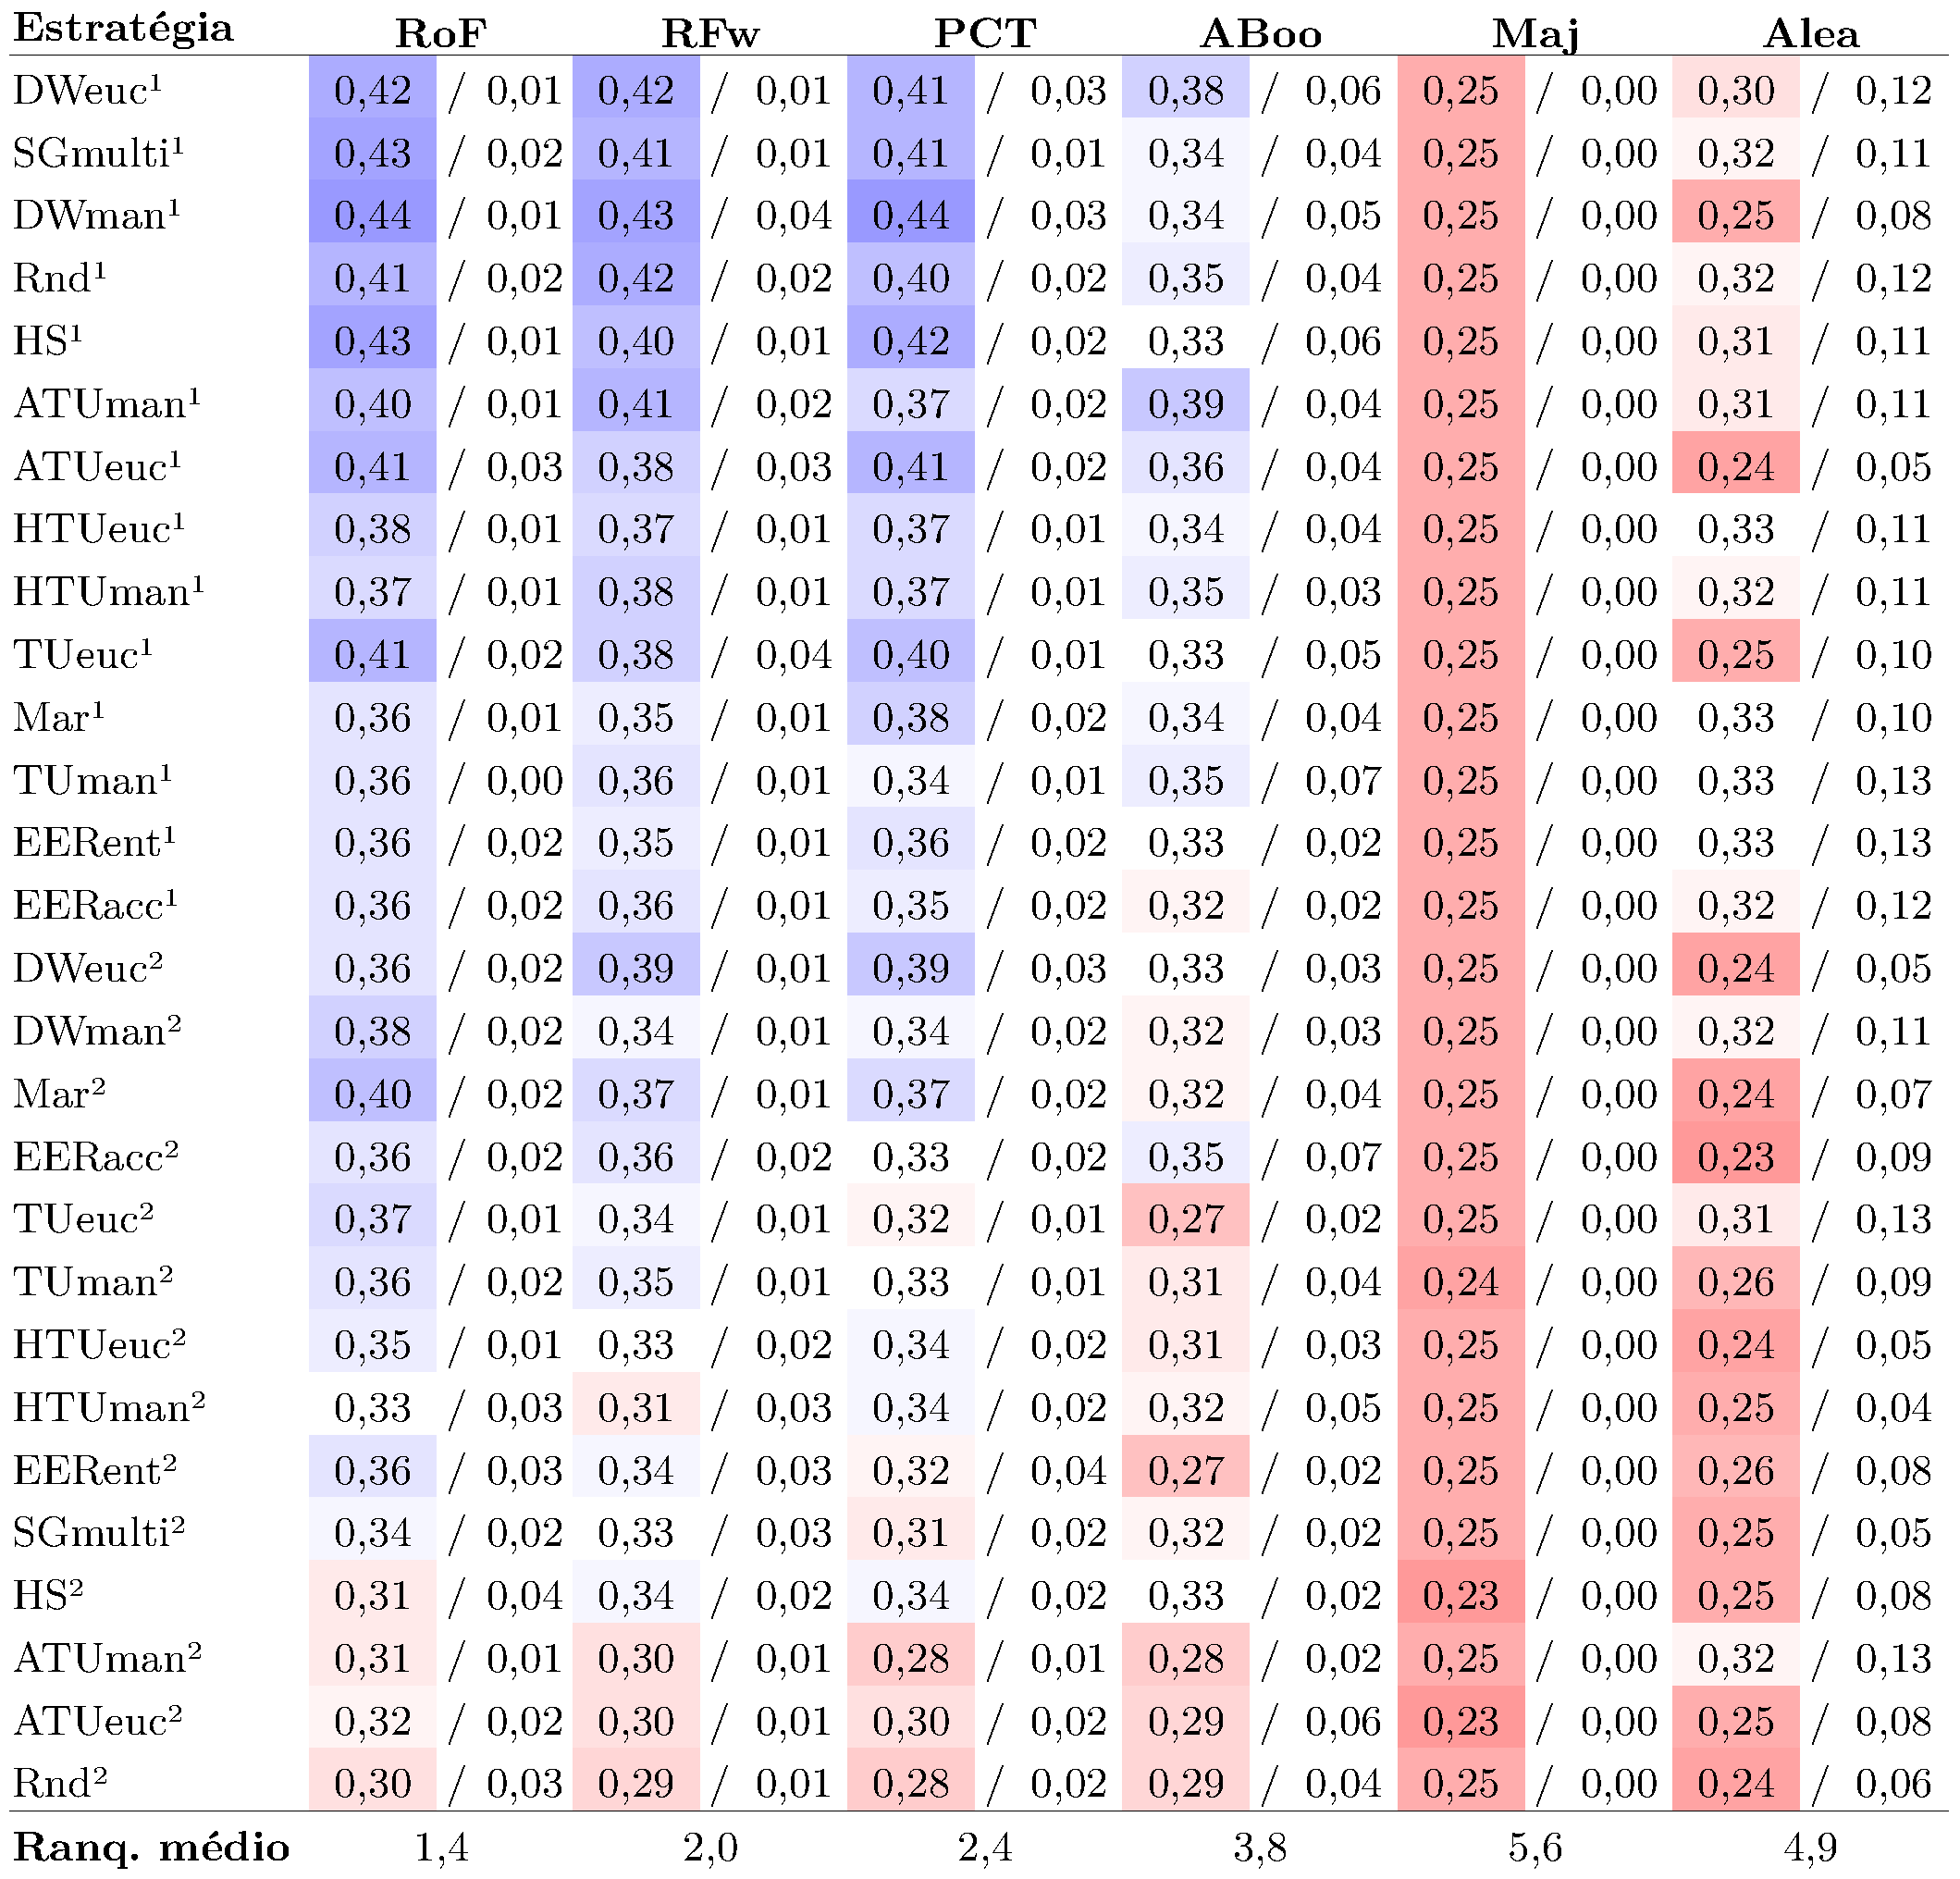
\includegraphics[scale=0.4]{images/metaacb.pdf}
\caption[Comparação da acurácia balanceada na recomendação do melhor algoritmo de aprendizado.]{Comparação da acurácia balanceada (média/desvio padrão) na recomendação do melhor algoritmo de aprendizado.
\textit{Detalhes na Figura \ref{accmeta}.}}
\label{accbalmeta}
\end{figure}

Finalmente, pode-se concluir que \destaque{o desempenho do sistema de recomendação proposto pode ser melhorado com a troca do meta-aprendiz, pois não se restringe ao uso do algoritmo PCT nesse papel}, embora ABoo, especificamente, tenha se mostrado pouco recomendável quando comparado aos demais, dentro das limitações impostas pelo arcabouço experimental.

Experimentos com outras modalidades de recomendação serão reportados na Seção \ref{outmod}.
Os meta-atributos são analisados a seguir, na Seção \ref{metaatts}.

\subsection{Análise dos meta-atributos}\label{metaatts}
\simbolo{G}{índice de  impureza de Gini}
% It is sometimes called "gini importance" or "mean decrease impurity" and is defined as the total decrease in node impurity (weighted by the probability of reaching that node (which is approximated by the proportion of samples reaching that node)) averaged over all trees of the ensemble. [do site SO]

É possível analisar quais aspectos são mais importantes na caracterização dos conjuntos de dados, por meio da quantificação da relevância de cada atributo para o meta-aprendiz.
Em comitês de árvores de decisão, a relevância\footnote{A implementação do algoritmo RF presente na biblioteca \textit{scikit learn} foi utilizada no cálculo da relevância de atributos \cite{scikit-learn}.} de cada meta-atributo \cite{books/wa/BreimanFOS84} é calculada por meio da média das reduções que ele causa na impureza, dadas pelas diferenças no \textit{índice Gini} entre nós pais e nós filhos durante a indução do meta-aprendiz RFw.
% ponderada pela probabilidade dele ser alcançado .
A impureza de cada nó é dada pelo índice Gini - conforme Equação \ref{gini}.
\begin{equation}\label{gini}
   G_n = \sum_{y \in Y} P_n(y) [1 - P_n(y)]
\end{equation}
A probabilidade $P_n(y)$ indica a proporção de exemplos da classe $y$ na sub-árvore representada pelo nó $n$.

A Tabela \ref{relev1} contém os valores de relevância dos meta-atributos em ordem decrescente.
% $$$
Os dois meta-atributos com os maiores valores de relevância são humanamente interpretáveis: percentual de atributos nominais ($\pno$) e quantidade máxima de atributos nominais ($\qnom_{max}$).
Os próximos cinco são medidas estatísticas a respeito da distribuição dos dados (entropia, curtose, correlação) e uma medida de agrupamento.
\begin{table}
\caption[Relevância dos meta-atributos]{Relevância dos meta-atributos na recomendação de algoritmos de aprendizado. \textit{Obtida para a primeira metade das consultas de HTUeuc com o meta-aprendiz RFw.}}
\label{relev1}
\parbox[t][]{.28\linewidth}{\vspace{0pt}
\centering
\scalebox{0.9}{\begin{tabular}{p{1.9cm}l}
\toprule
\textbf{Meta-atributo} & \textbf{Relevância} \\
\midrule
$\pno$	&	0,0389	\\
$\qnom_{max}$	&	0,0344	\\
$\en_{min}$	&	0,0307	\\
$\ku_{min}$	&	0,0294	\\
$\du_{k1}$	&	0,0279	\\
$\rho_{min}$	&	0,0278	\\
$\en_{mea}$	&	0,0273	\\
$\qnom_{mea}$	&	0,0271	\\
$\rho_{min/max}$	&	0,0257	\\
$\qnom_{min}$	&	0,0245	\\
$\cn_{h2}$	&	0,0235	\\
$\rho_{mea}$	&	0,0235	\\
${\mu}_{min}$	&	0,0228	\\
$\du_{k1.5}$	&	0,0224	\\
$\cn_{k1}$	&	0,0222	\\
$\du_{h1}$	&	0,0215	\\
$\si_{k2}$	&	0,0212	\\
$\sigma_{min}$	&	0,0212	\\
\bottomrule
\end{tabular}}
}
\hfill
\parbox[t][]{.3\linewidth}{\vspace{0pt}
\centering
\scalebox{0.9}{\begin{tabular}{p{1.9cm}l}
\toprule
\textbf{Meta-atributo} & \textbf{Relevância} \\
\midrule
$\du_{h1.5}$	&	0,0207	\\
$\sigma_{min/max}$	&	0,0196	\\
$\si_{h2}$	&	0,0195	\\
$\rho_{h}$	&	0,0193	\\
$\sk_{min}$	&	0,0189	\\
$\sk_{min/max}$	&	0,0187	\\
$\rho_{h1.5}$	&	0,0182	\\
$\du_{h2}$	&	0,0179	\\
$\si_{k}$	&	0,0176	\\
$\rho_{k1.5}$	&	0,0172	\\
$\qexeatt$	&	0,0169	\\
$\rho_{k2}$	&	0,0169	\\
$\lgqexeatt$	&	0,0169	\\
$\si_{h1.5}$	&	0,0165	\\
$\sigma_{mea}$	&	0,0163	\\
$\sk_{mea}$	&	0,0159	\\
$\qexe$	&	0,0157	\\
$\ku_{min/max}$	&	0,0154	\\
\bottomrule
\end{tabular}}
}
\hfill
\parbox[t][]{.28\linewidth}{\vspace{0pt}
\centering
\scalebox{0.9}{\begin{tabular}{p{1.9cm}l}
\toprule
\textbf{Meta-atributo} & \textbf{Relevância} \\
\midrule
$\du_{k2}$	&	0,0150	\\[1pt]
$\sigma_{max}$	&	0,0150	\\[1pt]
${\mu}_{mea}$	&	0,0149	\\[1pt]
$\si_{h}$	&	0,0147	\\[1pt]
$\si_{k1.5}$	&	0,0146	\\[1pt]
$\qatt$	&	0,0145	\\[1pt]
$\en_{max}$	&	0,0144	\\[1pt]
$\lgqexe$	&	0,0139	\\[1pt]
$\sigma_{min/max}$	&	0,0132	\\[1pt]
$\ku_{mea}$	&	0,0129	\\[1pt]
${\mu}_{min/max}$	&	0,0123	\\[1pt]
$\ku_{max}$	&	0,0119	\\[1pt]
${\mu}_{max}$	&	0,0119	\\[1pt]
$\qnc$	&	0,0113	\\[1pt]
$\sk_{max}$	&	0,0112	\\[1pt]
$\qnom_{min/max}$	&	0,0078	\\[1pt]
$\rho_{max}$	&	0,0005	\\[1pt]
\bottomrule
\end{tabular}}
}
\end{table}

A análise de uma árvore de decisão isolada permite verificar diretamente a distribuição das predições de acordo com os meta-atributos mais relevantes.
Uma árvore induzida pelo algoritmo (meta)C4.5w com no mínimo 10 exemplos por folha é apresentada na Figura \ref{treebonsalg}.
% ? -> -100
\begin{figure}
	\centering
	\includestandalone[mode=buildmissing]{treeBons}
	\caption[Árvore com os meta-atributos mais relevantes.]{Árvore com os meta-atributos mais relevantes de acordo com o meta-aprendiz C4.5w.}
	\label{treebonsalg}
\end{figure}
A árvore contém os meta-atributos mais relevantes. Ela foi induzida utilizando todos os metaexemplos.

Os meta-atributos, naturalmente, não coincidem totalmente com os mais relevantes segundo as estimativas do meta-aprendiz RFw (com 500 árvores), mas são igualmente representativos, dado o mesmo valor de acurácia (0,62) de (meta)C4.5w e RFw obtido na validação cruzada em dez partes.

Algumas observações podem ser feitas.
O algoritmo NB, seguido de C4.5w, obteve mais vitórias (15) do que todos os demais juntos (10) quando \textit{havia mais de um valor em atributos nominais} ($\qnom_{min}>1$).
Essa constatação é compatível com a natureza de NB e C4.5w, pois são capazes de processar atributos nominais diretamente - diferentemente de SVM e 5NNw.
O outro ramo da raiz agrupa os conjuntos que contêm apenas atributos numéricos, sendo que o algoritmo 5NNw obteve as 10 vitórias do caminho
$\qnom_{min}$ \MVRightarrow\phantom{i} $\mu{min}$ \MVRightarrow\phantom{i} $\qexeatt\leq 39,4$.
Outro caminho com clara capacidade discriminatória é $\qnom_{min}$ \MVRightarrow\phantom{i} $\mu{min}\leq 0,5$, em que apenas 5NNw (27) e NB (7) obtêm vitórias.
Em ambos os casos, não foi encontrada uma relação evidente entre o caminho e a folha.
Por fim, nota-se que o comitê RFw com 500 membros poderia, nesse caso, ser substituído por uma árvore isolada, como o (meta)C4.5w, sem perda de acurácia.
Apenas três meta-atributos foram suficientes para caracterizar os conjuntos de dados: $\qnom_{min}$, $\mu{min}$ e $\qexeatt$.
Uma característica comum entre eles é não serem medidas específicas de agrupamento de dados.

A presente análise não foi estendida à recomendação de pares devido à sua semelhança com a recomendação de algoritmos de aprendizado, causada pela forte influência do algoritmo no par.
Nas demais modalidades de recomendação, as árvores isoladas geradas pelo algoritmo (meta)C4.5w não superaram a acurácia de referência.

% Preferi correlação do que isso abaixo, pois abaixo é muito afetado pelo balanceamento das metaclasses.
% \subsection{Análise de taxa de acerto por conjunto de dados}\label{dss}
% A dificuldade imposta pelos conjuntos pode ser estimada pela taxa de acerto em cada metaexemplo, consideradas as dez execuções da validação cruzada.
% Por simplicidade, foi escolhido apenas o melhor meta-aprendiz e uma das melhores estratégias, RoF e HTUeuc, respectivamente.
% Na Figura \ref{dss}, a coluna \textit{Valor} indica a taxa de acerto por metaexemplo cujo conjunto de dados correspondente tem seu nome dado na primeira coluna.
% \begin{figure}
% \centering
% \includegraphics[scale=0.195]{images/dss.pdf}
% \caption[Taxas de acerto por conjunto de dados.]{Taxas de acerto por conjunto de dados}
% \label{dss}
% \end{figure}
% Essa taxa é calculada pela quantidade de acertos dividida por 10, que é o total de execuções da validação cruzada.
% A segunda coluna (\textit{\#sim}) contém a quantidade média de metaexemplos usados para treinamento cujos domínios são similares ao domínio do conjunto de dados indicado na primeira coluna.
% A coluna \textit{Média} contém apenas dois valores: a média das taxas de acerto para os metaexemplos com mais de zero similares no conjunto de treinamento e a média das taxas de acerto para os demais metaexemplos.
% 
% Na primeira metade das consultas, o maior valor médio das taxas de acerto ocorreu para os metaexemplos com maior quantidade de similares: 0,75 nas primeiras 33 linhas contra 0,61 para nas demais.
% Isso poderia sugerir que a coleção de conjuntos adotada estivesse elevando as medidas de desempenho por conta da existência de dependência entre as amostras (conjuntos de dados).
% Porém, há uma sobreposição entre esses valores quando considerado o desvio padrão (0,14 e 0,15).
% Além disso, na segunda metade das consultas, a situação se apresenta invertida, sugerindo a possibilidade de tratar-se de um artefato estatístico ou haver situações específicas em que a similaridade entre domínios influencia positivamente ou negativamente nas medidas de desempenho.
% 
% A Figura \ref{dss} também permite identificar os conjuntos de dados mais difíceis para a tarefa de recomendação de algoritmo de aprendizado ou, pelo menos, mais afetados por perturbações na composição da reserva de exemplos, de forma a apresentarem uma metaclasse diferente a cada execução.
% Essa última possibilidade é consistente com o fato de que o desempenho geral dos algoritmos se torna menos distinguível à medida que o aprendizado avança, conforme visto previamente na Figura \ref{curvasrankbands} no intervalo de consultas considerado. 
% 
